% xetex compatible variant that support TTF fonts according to company rules
\documentclass[ignorenonframetext, professionalfonts, hyperref={unicode}]{beamer}

\usetheme{Epam}

\usepackage{fontspec}
\setsansfont{SourceSansPro-Regular}
%\setbeamerfont{frametitle}{family=\fontspec{Oswald}}
\setbeamerfont{frametitle}{family=\fontspec{Oswald}}
\setbeamerfont{block title}{family=\fontspec{Oswald}}

%\setmainfont{Times New Roman}
\defaultfontfeatures{Mapping=tex-text}
\defaultfontfeatures{Ligatures=TeX}

%\setsansfont{Arial}
%\setromanfont{Trebuchet MS}

\usepackage{cmap}
\usepackage{graphicx}

\usepackage{textcomp}

\usepackage{beamerthemesplit}

\usepackage{ulem}

\usepackage{verbatim}
\usepackage{import}

\usepackage{listings}
\lstloadlanguages{bash}

\lstset{escapechar=`,
	captionpos=b,
	extendedchars=false,
	language=sh,
%	frame=single,
	tabsize=2, 
	columns=fullflexible, 
%	basicstyle=\scriptsize,
	keywordstyle=\color{blue}, 
	commentstyle=\itshape\color{brown},
%	identifierstyle=\ttfamily, 
	stringstyle=\mdseries\color{green}, 
	showstringspaces=false, 
	numbers=left, 
	numberstyle=\footnotesize, 
	breaklines=true, 
	inputencoding=utf8,
	keepspaces=true,
	morekeywords={u\_short, u\_char, u\_long, in\_addr}
	}

\definecolor{darkgreen}{cmyk}{0.7, 0, 1, 0.5}

\lstdefinelanguage{diff}
{
    morekeywords={+, -},
    sensitive=false,
    morecomment=[l]{//},
    morecomment=[s]{/*}{*/},
    morecomment=[l][\color{darkgreen}]{+},
    morecomment=[l][\color{red}]{-},
    morestring=[b]",
}

\author[Epam]{{\bf Epam}\\Low Level Programming Department}

%\institution[EPAM]{EPAM}
%\logo{\includegraphics[width=1cm]{logo.png}}

\graphicspath{{../../slides/cmdline/clipart/}{../../slides/bash/clipart/}}

\bibliographystyle{unsrt}
\setbeamertemplate{bibliography item}{\insertbiblabel}

\AtBeginSection[]{%
  \begin{frame}<beamer>
    \frametitle{}
    \tableofcontents[
        sectionstyle=show/shaded, hideallsubsections ]
  \end{frame}
  \addtocounter{framenumber}{-1}% If you don't want them to affect the slide number
}

% \regex for regular expressions
\newcommand{\regex}[1]{ %
\expandafter{$\ulcorner{\color{blue}\texttt{#1}}\lrcorner$} %
}



\title{Введение в GNU/Linux}


%%%%%%%%%%%%%%%%%%%%%%%%%%%%%%%%%%%%%%%%%%%%%%%%%
%%%%%%%%%% Begin Document  %%%%%%%%%%%%%%%%%%%%%%
%%%%%%%%%%%%%%%%%%%%%%%%%%%%%%%%%%%%%%%%%%%%%%%%%

\begin{document}

\begin{frame}
	\frametitle{}
	\titlepage
	\vspace{-0.5cm}
	\begin{center}
	%\frontpagelogo
	\end{center}
\end{frame}


\begin{frame}
	\tableofcontents
	[hideallsubsections]
\end{frame}

\section{О курсе}

\mode<all>{\begin{frame}{About myself.}

    \large Vikentsi Lapa - Senior Software Test Automation Engineer
    \begin{columns}
        \column{0.6\textwidth}
            \begin{itemize}
                \item Hands on experience with Linux about 8 years in such areas as
                \begin{itemize}
                    \item High Perfomance Computing
                    \item Cluster file systems: GPFS, Lustre 
                \end{itemize}
                \item MLUG (Minsk Linux User Group Activist) and LVEE conference participant 
            \end{itemize}
        \column{0.3\textwidth}
            \center
\includegraphics[width=3cm]{myphoto}
    \end{columns}
\end{frame}

\begin{frame}{Cложность изучения системы.}
         \center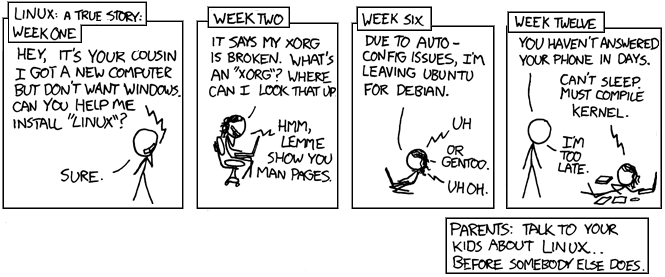
\includegraphics[scale=0.6]{linux_story} 
    \break
\pause
Сложности: множество вариантов, обилие информации, терминология, новые интерфейсы, ошибки.
\pause
	\begin{center}
		\large
		Обеспечить быстрый старт в среде GNU/Linux для опытных пользователей. Понизить порог вхождения. Задать направление. 
	\end{center} 
\end{frame}


\begin{frame}{Аудитория}

Кому полезен этот курс:
\begin{itemize}
    \item IT Engineers, DevOps Engineers
    \item Junior Software Engineers/Software Engineers
    \item Test Engineers, Test Automation Engineers
    \item Students
\end{itemize}
    \pause
Что требуется от вас:
\begin{itemize}
    \item Опыт работы с Linux/Unix меньше 1 года или без опыта
    \pause
    \item Опыт работы с системой виртуализации
    \item Знание сетевых технологий
    \item Creative thinking and problem solving skills
    \pause
    \item \alert{Feedback is essential: answer to questions, do practical tasks, do homework, ask questions}
\end{itemize}
\end{frame}

\begin{frame}{Проверим обратную связь}
\begin{itemize}
    % this one moved to email trainee introduction
    %\item Есть ли опыт работы с Linux? Если есть то сколько?
    %\pause
    %\item Ваши ожидания. Зачем пришли на курс?
    %\pause
    \item Установили дистрибутив? Какой?
    \item Если не установили напишите причину.
\end{itemize}
\end{frame}

\begin{frame}[fragile]{Оценка возраста системы Unix.}
Ваша версия.
 \pause
\begin{lstlisting}
    $ date --help | grep '%s'
    $ date +%s # show current date in seconds 
    $ echo $(( $(date +%s)/(60*60*24*365))) # show years
\end{lstlisting} 
\pause
Unix systems are characterized by a \alert{modular design} or ``Unix philosophy"
		\begin{columns}
		\column{0.7\textwidth}
\begin{itemize}
    \item simple tools that each perform a limited, well-defined function
    \item shell scripting and command language to combine the tools to perform complex workflows
    \item unified filesystem
\end{itemize}
		\column{0.3\textwidth}
            
\includegraphics[width=4cm]{40years}
		\end{columns}
% За это время сложилась культура и философия разработки, которая оказала влияние на интерфейсы взаимодействия, например названия устройств и команд.
% Разнообразие подходов при решении задач. Среда дружественная для программиста и опытного технического пользователя.
\end{frame}


%\begin{frame}{Состав курса}
%	\begin{itemize}
%		\item Представление об архитектуре GNU/Linux дистрибутива
%			\pause
%		\item "Ежедневные" навыки работы в консоли. Конфигурация системы.
%			\pause
%		\item Язык программирования
%			\begin{itemize}
%					\item shell (Bash)
%			\end{itemize}
%			\pause
%		\item Все, чего вы не знали и боялись спросить
%	\end{itemize}
%\end{frame}
}


%%%%%%%%%%%%%%%%%%%%%%%%%%%%%%%%%%%%%%%%%   
%%%%%%%%%% Content starts here %%%%%%%%%%
%%%%%%%%%%%%%%%%%%%%%%%%%%%%%%%%%%%%%%%%%

\section{Дистрибутивы ОС Linux}
\mode<all>{\begin{frame}{Дистрибутив ОС GNU/Linux}
	\begin{block}{ Определение}
		\only<1>{\center{\bf{?}}}
		\pause
		\only<2->{Набор программного обеспечения на базе ядра Linux, распространяющийся как единое целое.}
	\end{block}
\end{frame}


\begin{frame}{Задачи дистрибутива}
	\begin{itemize}
		\item Предоставление комплекта ПО (ядро + утилиты)
		\item Средства установки и настройки
		\item Средства обновления
	\end{itemize}
\end{frame}

\begin{frame}{Различия между дистрибутивами}

	\only<1>{\Large\center{\bf{?}}}
	\pause
	\only<2->{\Large\center{\bf{Цели!!!}}}

	\bigskip
	\normalsize

	\pause

	\begin{itemize}
		\begin{columns}
		\column{0.4\textwidth}
			\item Инсталлятор
			\item Первичные настройки
			\item Средства управления
			\item Набор ПО
		\column{0.4\textwidth}
			\item Менеджер пакетов
			\item Формат распространения ПО
			\item Пути к файлам
			\item Система сборки ПО
		\end{columns}
	\end{itemize}
\end{frame}

\begin{frame}{Дистрибутивы}
	\begin{itemize}
		\begin{columns}
		\column{0.3\textwidth}
			\item RedHat
			\item Fedora Core
			\item CentOS
			\item Scientific Linux
			\item Oracle Unbreakable Linux
		\column{0.3\textwidth}
			\item Slackware 
			\item Gentoo
			\item Arch
			\item OpenSUSE
			\item ALT Linux 
		\column{0.3\textwidth}
			\item Debian
			\item Ubuntu
			\item Mint
			\item Knoppix
			\item BackTrack
		\end{columns}
	\end{itemize}
\end{frame}
}

\section{Процесс загрузки ОС Linux}
\subsection{Этапы загрузки}
\mode<all>{\begin{frame}{Процесс загрузки GNU/Linux}
	\scriptsize
	\begin{enumerate}
		\item BIOS
		\item Master Boot Record (MBR)
			\pause
		\item Загрузка загрузчика 
		\begin{itemize}
		\footnotesize
			\item Stage 1 -- Первичный загрузчик
			\item Stage 1,5 -- Загрузка ядра загрузчика и драйвера ФС
			\item Stage 2 -- загрузчик читает конфигурацию, загружает ядра и образ initrd (initial-RAM disk) в память
                        \item Передает управление ядру
		\end{itemize}

		\item Запуск программы инициализации в initrd, загрузка драйверов файловых систем (LVM, RAID, NFS)
			\pause
		\item Нахождение и монтирование корневого раздела
			\pause
		\item Запуск программы init
		\begin{itemize}
		\footnotesize
			\item Монтирование оставшихся разделов ФС
			\item Запуск демонов для заданного уровня загрузки (runlevel)
			\item Выдает приглашение пользователю. 
		\end{itemize}

	\end{enumerate}
\end{frame}
}

\subsection{Ядро Linux}
\mode<all>{\begin{frame}{Задачи ядра Linux}
	\begin{itemize}
		\item Инициализация системы
		\item Управление процессами и потоками
		\item Управление памятью
		\item Управление файлами
		\item IPC (Inter Process Communication)
		\item Разграничение доступа
		\item Сетевые возможности
		\item Интерфейс доступа к возможностям ядра
	\end{itemize}
	%Выполнить команду dmesg и найти строки инициализации памяти, CPU, дисковой подсистемы, CPU.
\end{frame}


\begin{frame}{Ядро}

	Ядро ОС Linux является модульным. 

	\begin{block}{Модули}
		\begin{itemize}
			\item В виде отдельных файлов
			\item "Вкомпилированные" в ядро
		\end{itemize}
	\end{block}

	\bigskip
	%Список загруженных модулей: {\tt cat /proc/modules } либо {\tt lsmod}
\end{frame}


\begin{frame}{Параметры ядра}
	
	Полный список: {\tt Documentation/kernel-parameters.txt}

	\begin{block}{Некоторые часто применяемые параметры}
		\begin{itemize}
			\begin{columns}
			\column{0.3\textwidth}
				\item console=ttyS0,9600
				\item debug
				\item init=/sbin/init
				\item loglevel=[0-7]
				\item maxcpus=[num]
			\column{0.3\textwidth}
				\item mem=nn[KMG]
				\item noacpi
				\item noapic
				\item panic=nn (sec)
				\item resume=/dev/sda2
			\column{0.3\textwidth}
				\item ro
				\item rw
				\item root=/dev/sda1
				\item rootdelay=nn (sec)
				\item rootwait
				\item vga=<num>|ask
			\end{columns}
		\end{itemize}
	\end{block}

	Параметры переданные ядру во время загрузки: {\tt /proc/cmdline} \\

        Программы могут использовать /cmdline, например установщик ОС Anaconda \\

	Модулям можно передавать параметры используя синтаксис: {\tt module.param=value} \\
\end{frame}
}

%\subsection{Система инициализации.}
%\mode<all>{\begin{frame}{init}
	Менеджер управления работой системой и сервисами.
	
	\bigskip

	\center{\large PID = 1}

	\bigskip

	\begin{block}{Наиболее известные}
		\begin{itemize}
			\item SysVInit
			\item systemd
			\item upstart
		\end{itemize}
	\end{block}
\end{frame}

\begin{frame}{SysVInit}
	\begin{block}{Управление}
		\begin{itemize}
			\item kernel boot parameters: <N> -- runlevel
			\item утилита {\tt runlevel}
			\item утилита {\tt init}
		\end{itemize}
	\end{block}

	\scriptsize
	\begin{block}{Runlevel}
		\begin{table}
			\begin{tabular}{| c | l | }
			\hline
			Runlevel & Описание\\
			\hline
			0	& Выключить систему \\
			1,s,single & Однопользовательский режим \\
			2	& Многопользовательский режим без графики. Без сетевых сервисов.\\
			3	& Многопользовательский режим без графики. Полноценная сеть. \\
			4	& Определяется на хосте\\
			5	& Многопользовательский режим с графикой.\\
			6	& Перезагрузка\\
			emergency & Аварийная оболочка \\
			\hline
			\end{tabular}
		\end{table}
	\end{block}
\end{frame}

\begin{frame}{SysVInit: сервисы}
	\begin{block}{Управление}
		\begin{itemize}
			\item утилита {\tt service}
			\item утилита {\tt chkconfig}
		\end{itemize}
	\end{block}

	\begin{block}{Сервисы}
		\begin{itemize}
			\item {\tt /etc/rc.d/init.d}
			\item {\tt /etc/rc.d/rc.N}\footnote{N=runlevel}
		\end{itemize}
	\end{block}
\end{frame}

\begin{frame}{systemd}
	\begin{block}{Управление}
		\begin{itemize}
			\item kernel boot parameters\\
				{\tt systemd.unit=rescue.target} \\
			\item утилита {\tt systemctl} \\
				{\tt systemctl isolate multi-user.target} \\
				{\tt systemctl set-default single.target}
		\end{itemize}
	\end{block}

	\begin{block}{targets}
		\tiny
		\begin{table}
			\begin{tabular}{| c | l | l | }
			\hline
			Runlevel & Описание\\
			\hline
			0	& poweroff.target & Выключить систему \\
			1,s,single & rescue.target  & Однопользовательский режим \\
			2	& multi-user.target & Многопользовательский режим без графики. Без сетевых сервисов.\\
			3	& multi-user.target & Многопользовательский режим без графики. Полноценная сеть. \\
			4	& multi-user.target & Определяется на хосте\\
			5	& graphical.target & Многопользовательский режим с графикой.\\
			6	& reboot.target & Перезагрузка\\
			emergency & emergency.target & Аварийная оболочка \\
			\hline
			\end{tabular}
		\end{table}
	\end{block}
\end{frame}

\begin{frame}{systemd: сервисы}
	\begin{block}{Управление}
		\begin{itemize}
			\item утилита {\tt systemctl}
		\end{itemize}
	\end{block}

	\begin{block}{Сервисы}
		\begin{itemize}
			\item {\tt /lib/systemd/system/}
			\item {\tt /etc/systemd/system/}
		\end{itemize}
	\end{block}
\end{frame}
}

\section{Вход в систему.}
\mode<all>{% пользовательская сессия
\begin{frame}
  \frametitle{Пользовательская сессия}

  \begin{center}
    \begin{block}<1->{Многопользовательская система?}
      Надо представиться системе. Логин и пароль.
    \end{block}

    \begin{block}<2->{Как может выглядеть}
      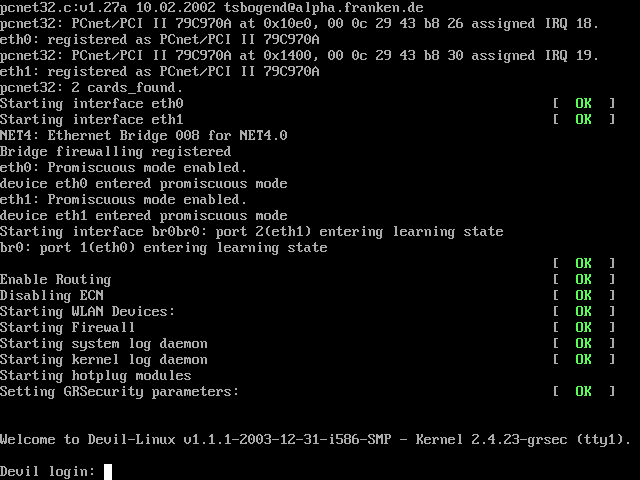
\includegraphics[height=2.5cm]{console-login-screenshot}
      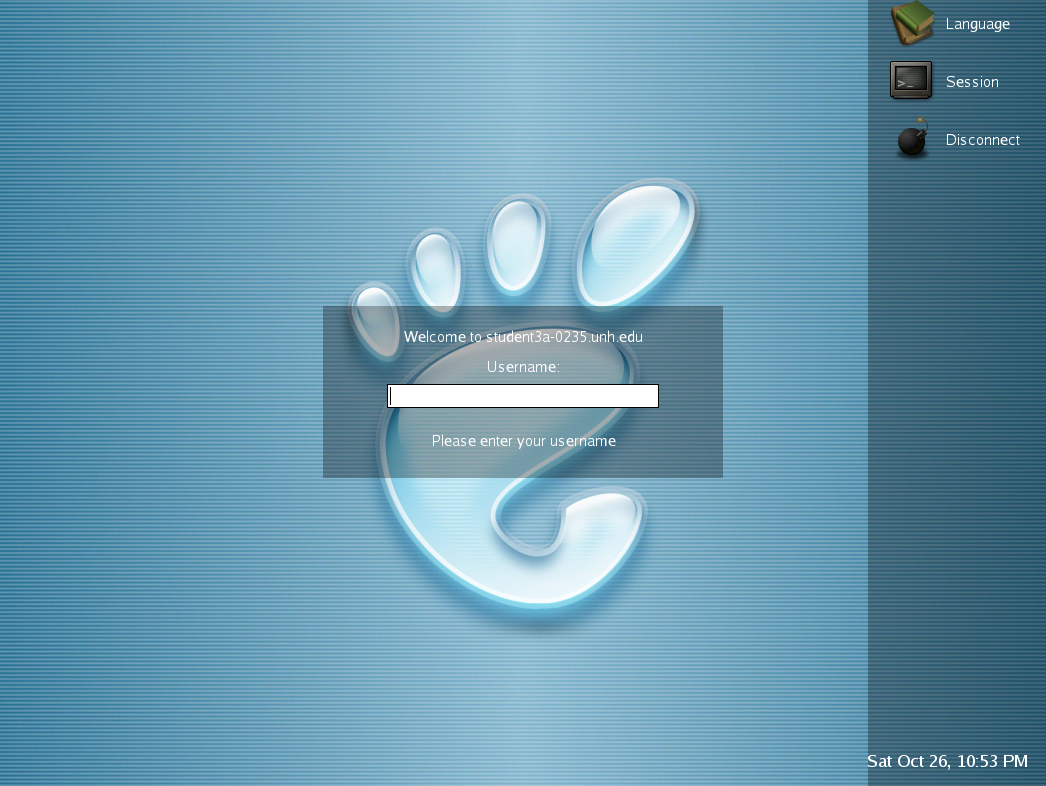
\includegraphics[height=2.5cm]{gdm-login-screenshot}
      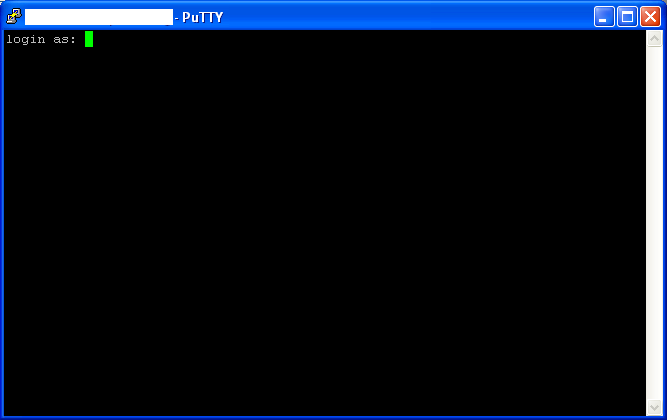
\includegraphics[height=2.5cm]{putty-login-screenshot}
    \end{block}

    \begin{block}<3->{Виды сессий}
      \begin{itemize}
        \item локальные и удалённые (сетевые)
        \item текстовые и графические
      \end{itemize}
    \end{block}

  \end{center}

\end{frame}

\begin{frame}
  \frametitle{Входим удалённо. SSH}

  \begin{center}

    SSH - \emph{S}ecure \emph{SH}ell
    \newline \pause

    Протокол удалённой работы по сети для Linux.

    Много реализаций клиентов и серверов.
    \newline
    \pause

    \emph{Как может выглядеть:}
    \newline
    \fbox{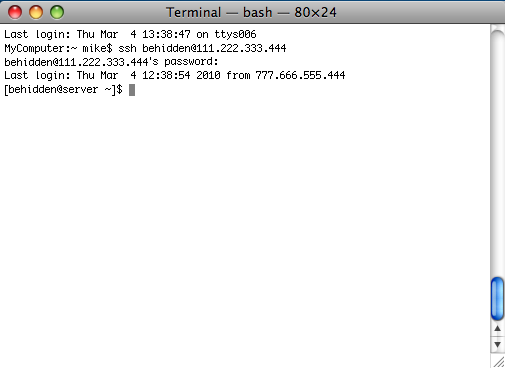
\includegraphics[height=3.5cm]{console-ssh-screenshot}}
    \emph{ }
    \fbox{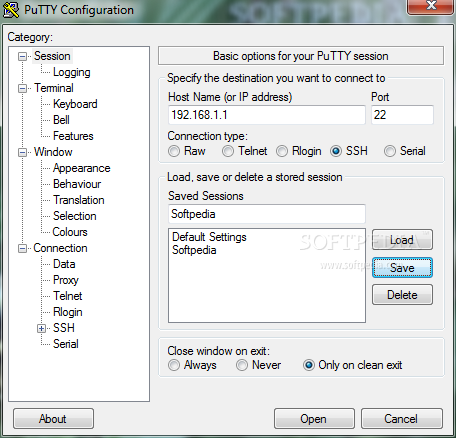
\includegraphics[height=3.5cm]{putty-config-screenshot}}
  \end{center}

\end{frame}

\begin{frame}
  \frametitle{Выход из матрицы}

  \begin{center}
    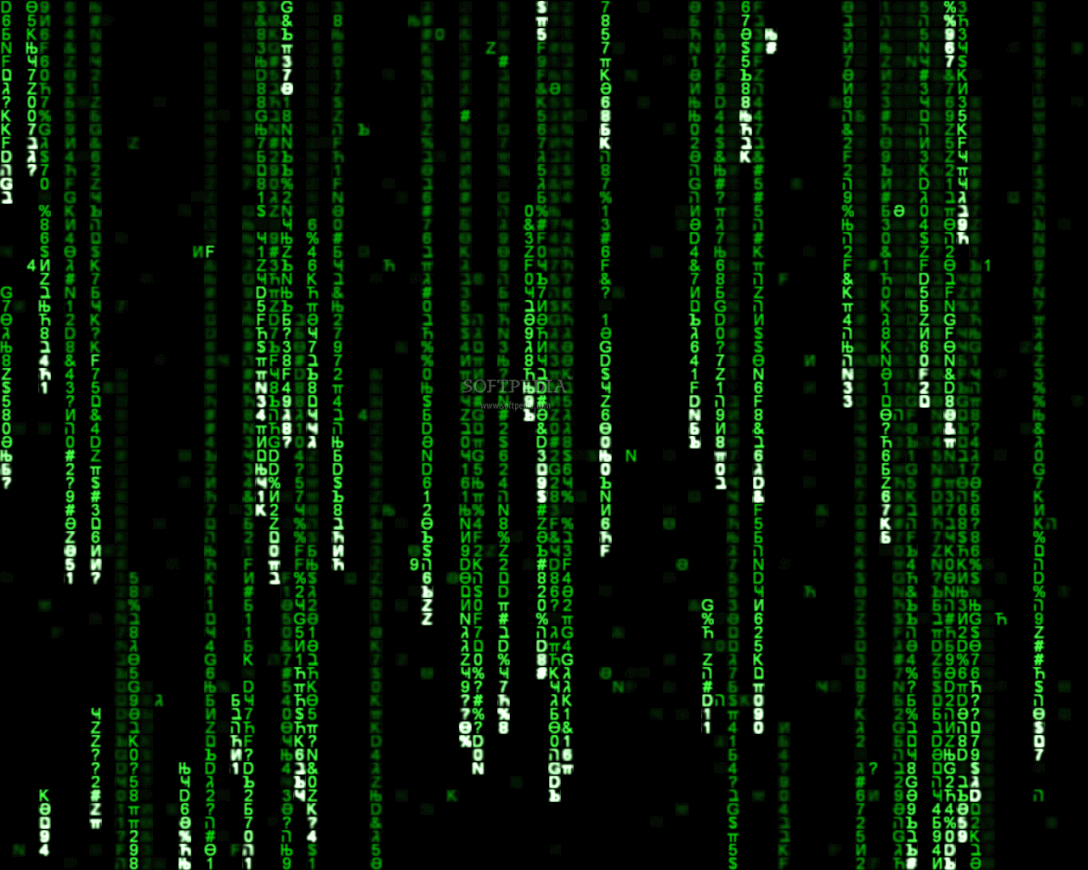
\includegraphics[height=5.5cm]{matrix-screenshot}
    \pause
    \newline
    \begin{itemize}
      \item Команда \emph{exit}
      \item Команда shell \emph{logout}
      \item Hotkey \emph{Ctrl+d}
      \item Закрыть клиента
    \end{itemize}
  \end{center}

\end{frame}
}
\subsection{Беспарольный вход}
\mode<all>{\begin{frame}
  \frametitle{Методы авторизации SSH. Ключи}

  \alert{Не хочешь вводить пароли?}
  \pause

  \alert{Не вводи!}
  \pause

  \begin{center}
    Aвторизация в SSH.

    Пара: открытый + секретный ключ.

    Вместо пароля.
  \end{center}

\end{frame}

\begin{frame}
  \frametitle{Ключи SSH. Создание}

  \begin{center}

    \begin{tabular}{ l r }
      \hbox{Linux: ssh-keygen} & \hbox{Windows: PuTTY keygen} \\
      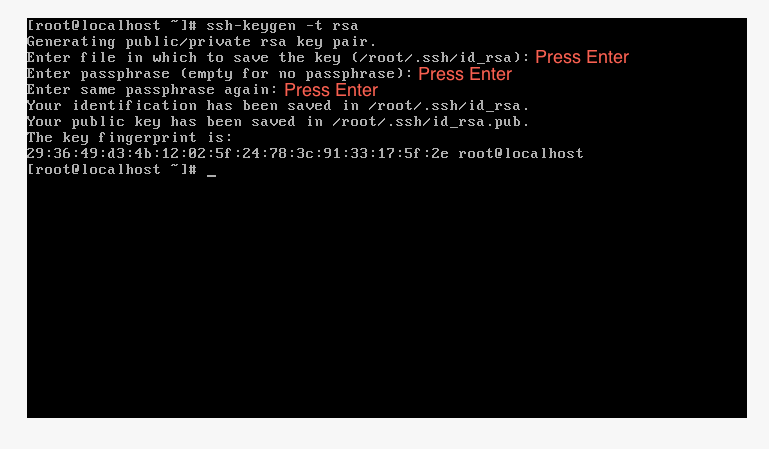
\includegraphics[height=3cm]{ssh-keygen-screenshot} & 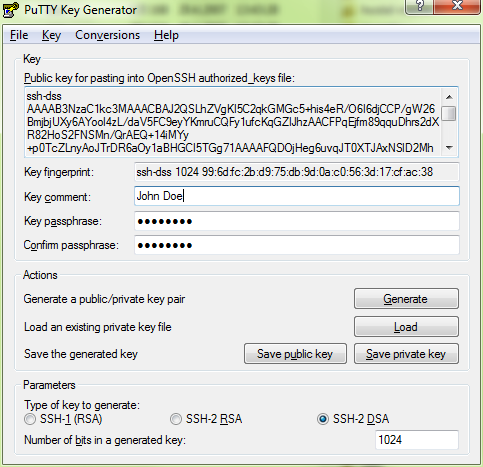
\includegraphics[height=4cm]{putty-keygen-screenshot} \\
      Ключи в папке .ssh/: & Ключи там, где сохранили \\
      id\_rsa и id\_rsa.pub &
    \end{tabular}

  \end{center}

\end{frame}


\begin{frame}
  \frametitle{Ключи SSH. Копирование}

  \begin{itemize}
    \item \alert{Что копировать?} Публичный ключ (id\_rsa.pub)  \pause
    \item \alert{Куда складывать?} в \$HOME/.ssh/authorized\_keys \newline удалённой машины \pause
    \item \alert{Как перенести?} \pause
      \begin{itemize}
        \item Linux: ssh-copy-id username@host \pause
        \item Copy-paste в редактор \pause
      \end{itemize}
  \end{itemize}

\end{frame}

\begin{frame}
  \frametitle{SSH. Автоматизация входа}
  \begin{center}
    \begin{tabular}{ l r }
      \Large{Linux: .ssh/config} & \Large{Windows: PuTTY session} \\
      \lstinputlisting[basicstyle=\tiny]{../../sam-solutions/samples/ssh-config} & \fbox{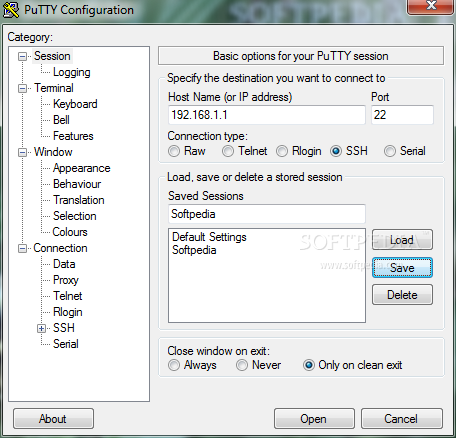
\includegraphics[height=4.3cm]{putty-config-screenshot}} \\
    \end{tabular}

  \end{center}
\end{frame}
}

\section{Интерфейс командной строки}
\mode<all>{% Тема. Командная строка. 
% Показать примеры использования. Рассказать о преимуществах и недостатках в
% сравненни с графическим "оконным" интерфейсом. 
% Ознакомить с назначениме  эмулятора терминала и об реализациях.

\begin{frame}{Примеры использования командной строки}
        CLI (Command Line Interface)
	\begin{columns}
	\column{0.5\textwidth}
        \begin{itemize}
            \item интерфейс настройки сетевого оборудования
            \item чаты
            \item компьютерные игры
            \item операционные системы
        \end{itemize}
	\column{0.5\textwidth}
	% insert picture of Quake 
    \includegraphics[height=0.4\textheight]{../../slides/cmdline/330px-Tremulous_console.png}
	\end{columns}
\end{frame}

\begin{frame}{Преимущества командной строки}
	\begin{itemize}
                \item Используют мало ресурсов
		\item Работа через сеть либо RS232, в том числе медленную
		\item Быстрый доступ к командам системы
		\item Отладка сообществом CLI приложения проще
		\item Легкость автоматизации
	\end{itemize}
\end{frame}

\begin{frame}{Недостатки командной строки}
	\begin{itemize}
		\item Oтсутствуют возможности обнаружения (discoverabililty)
		\item Отсутствие «аналогового» ввода.
		\item Необходимость изучения синтаксиса команд и запоминания сокращений.  (синтаксис может различаться)
		\item Без автодополнения, ввод длинных и содержащих спецсимволы параметров с клавиатуры может быть затруднительным
	\end{itemize}
\end{frame}

\note { 
Примеры приложений которые лучше выглядят в графическом режиме браузер,
редакторы видео и графики. Поэтому пользователь при работе, как правило,
совмещает оба интерфейса: использует графическое окружениe в сочетании с
интерфейсом командной строки. 
В графическом окружении интерфейса командной строки предоставляют приложения -
эмуляторы терминала. 
реализации - для графической системы X Window xterm, rxvt. Для GNOME
gnome-terminal, для KDE konsole, Yakuake (Yet Another Kuake выезжает по нажатии
тильды ~ как Quake)  
Дополнительные замечания:
Терминал - устройство для ввода вывода информации, уже устарел.
Графические приложения можно запускать из командной строки. 
}
}

\section{Получение помощи}
\mode<all>{\begin{frame}[fragile]{From FAQ How To Ask Questions The Smart Way}
Before You Ask try to find an answer
  \begin{itemize}
	  \item by reading (RTFM): manual, FAQ, archives of the forum, by searching the Web;
	  \item by inspection or experimentation;
	  \item by asking a skilled friend;
	  \item by reading the source code;
    \end{itemize}
\end{frame}


\begin{frame}[fragile]{Встроенная документация}
\begin{itemize}
    \item \textbf{man} - помощь по внешним командам
    \pause
    \item \textbf{info} - расширенная помощь по некоторым командам (texinfo format)
    \pause
    \item \textbf{find /usr/share/doc/} - файлы документации поставляемые вместе с приложением
    \item \textbf{-h, --help option} - встроенная в приложение справка
    \item \textbf{help} - встроенная помощь по внутренним командам bash (также man bash)
\end{itemize}
\end{frame}

\begin{frame}[fragile]{Основное о man}
      \textbf{man \textless command\_name\textgreater }

	\begin{block}{Example: show uptime manual page}
		{\tt man uptime}
	\end{block}

		\begin{itemize}
			\item Прочитайте {\tt man man} !
		\end{itemize}

\end{frame}

\begin{frame}[fragile]{man page navigation}
		\begin{itemize}
			\item \textbf{up, down} - scroll one line
			\item \textbf{q} - exit
			\item \textbf{/pattern} - search pattern
			\item \textbf{n} - next text pattern
			\item \textbf{N} - repeat search in back direction
			\item \textbf{h} - help
		\end{itemize}
\end{frame}

\begin{frame}[fragile]{Page structure}
		\begin{itemize}
			\item NAME
			\item SYNOPSIS
			\item DESCRIPTION
			\item EXAMPLES
			\item SEE ALSO
		\end{itemize}
\end{frame}

\begin{frame}[fragile]{Разделы помощи}
	\begin{itemize}
		\item[1] Основная секция(юзерские программы)
		\item[2] Syscalls
		\item[3] С library
		\item[5] Конфигурационные файлы
		\item[8] Системные службы
	\end{itemize}
\end{frame}

\begin{frame}[fragile]{More than one section of the manual}
	name(section)  \\ 
	\textbf{man(1)} and \textbf{man(7)}, or \textbf{exit(2)} and \textbf{exit(3)} \\
     \begin{block}{Example: show manual in section 5 and 1}
        \begin{lstlisting}
man -f passwd #or whatis passwd 
man 5 passwd; man 1 passwd; man -wa passwd
        \end{lstlisting}
    \end{block}
\end{frame}

\begin{frame}[fragile]{Поиск по страницам помощи}
     \begin{block}{Упражнение. Поиск страниц с ключевым словом.}
        \begin{lstlisting}
man -f passwd #or whatis passwd 
man -k passwd #or apropos passwd 
whatis  -l -w '*'
man -s 3 -Kw passwd
        \end{lstlisting}
    \end{block}
\end{frame}


%\begin{frame}[fragile]{Чему научились}
%  \begin{itemize}
%  \item Как спрашивать у сообщества
%  \item Умеем использовать 3 источника получения информации man, info, help
%  \item Как перемещаться по страницам помощи info и man
%  \item Иcкать в системе помощи man и запрашивать из одного из 8-ми разделов 
%  \end{itemize}
%\end{frame}
}


\section{Навигация по файловой системе}
\mode<all>{\begin{frame}[fragile]{Путь к файлу.}
      \begin{itemize}
        \item Имя файла
                \begin{itemize}
                    \item чувствительно к регистру
                    \item / разделяет директории
                    \item - \textbackslash <Space> специальные символы 
                    \item . скрытый файл
                \end{itemize}
        \item \alert{Полное имя файла} (absolute pathname) начинается с /
        \item \alert{Относительное имя файла} (relative pathname) начинается с
        любого другого символа. Поиск файла производится относительно
        \alert{текущей директории} (current working directory).
      \end{itemize}

      \begin{block}{Примеры}
        ./ - текущая директория

        ../ - предыдущая директория

        ../../usr/bin/ls

        /usr/bin/ls
      \end{block}
\end{frame}

\begin{frame}[fragile]{Навигация по файловой системе}
      \begin{itemize}
		  \item {\tt pwd} -- имя текущей директории (help pwd)
		  \item {\tt ls} -- список файлов в директории. По умолчанию в текущей (man ls)
		  \item {\tt cd} -- смена текущей директории (help cd)
      \end{itemize}
      \begin{block}{Упражнение. Заходим в /usr/bin/ и просматриваем список доступных команд.}
	\begin{lstlisting}
	pwd
	cd /usr/bin/
	pwd
	ls
	cd -	
	pwd
	\end{lstlisting}
      \end{block}
\end{frame}

\begin{frame}[fragile]{Просмотр типов файлов}
      \begin{block}{Упражнение. Символьное обозначение типа файла.}
Первая буква вывода команды ls -l обозначает тип файла. 
Tip. Команды file позволяет определить тип файла. Ключ -d для работы с
директорией. 

/dev/zero

/dev/sda 

.. 

/bin/sh 

/dev/log

/dev/stdout
      \end{block}
\end{frame}

\begin{frame}[fragile]{Команды для работы с файлами}
	\begin{itemize}
		\begin{columns}
		\column{0.2\textwidth}
			\item touch
			\item ln
			\item mkdir
			\item mknod
			\item mkfifo

		\column{0.2\textwidth}
			\item cp
			\item mv
			\item rm
			\item rmdir
			\item file
			\item install

		\column{0.4\textwidth}
			\begin{block}{Упражнение}
				\begin{enumerate}
					\item Создать иерархию директорий
						\begin{lstlisting}
dir1/dir1.1/dir1.1.1
dir1/dir1.2/dir1.2.1
dir1/dir1.2/dir1.2.2
						\end{lstlisting}
					\item Внутри каждой создать файл
					\item Удалить все созданное
				\end{enumerate}
			\end{block}
			
		\end{columns}
	\end{itemize}
\end{frame}
}
\mode<all>{
\begin{frame}{Детали реализации}
  \begin{itemize}
    \item \alert{VFS - virtual file system} - файлы и каталоги отображаются в единое дерево, независимо от их физического расположения.
  \end{itemize}
  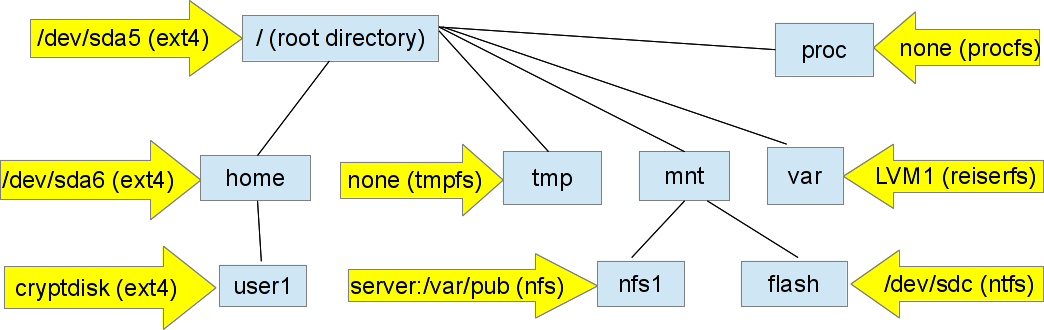
\includegraphics[height=3.5cm]{vfs-and-devices}
\end{frame}

\begin{frame}{Монтирование}
  \begin{itemize}
    \item \alert{Монтирование} - процесс отображения содержимого устройства в указанную папку файловой системы.
    \item Команды:
      \begin{itemize}
        \item монтировать - ( \alert{mount} ) 
        \item размонтировать ( \alert{umount} )
      \end{itemize}
    \item \alert{mount} без параметров - вывести список уже подключенных файловых систем
  \end{itemize}
      \begin{block}{Упражнение. Дерево монтирования.}
     Получить вывод смонтированных блочных устройств в виде дерева с помощью команды: \alert{findmnt}
      \end{block}
  
\end{frame}

}

\section{Интерактивная работа в командной оболочке (shell)}
\mode<all>{\begin{frame}{Делаем жизнь в консоли приятной}
  \begin{itemize}
	\item Меньше ошибок
	\item Легче вспомнить 
	\item Быстрее набрать и отредактировать
  \end{itemize}
\end{frame}

\begin{frame}{Автодополненение}
  Клавиша \textbf{Tab} 
  \begin{itemize}
	\item напоминалка имени команды и аргументов;
	\item файловый менеджер;
	\item ускоритель ввода.
  \end{itemize}
\end{frame}

\begin{frame}{История команд}
  Просмотреть историю \alert{{\tt history}}
  \begin{itemize}
	\item ближняя
	      \begin{itemize}
		\item Клавиши курсора, \alert{Ctrl-P}, \alert{Ctrl-N} -- навигация по истории
	      \end{itemize}
	\item дальняя 
	      \begin{itemize}
		\item \alert{\$ !10}  -- по номеру команды
		\item \alert{Ctrl-R} -- поиск в истории по фрагменту
	      \end{itemize}
	\item часть команды 
	      \begin{itemize}
		\item \alert{Alt-.}  -- последний аргумент предыдущей команды
	      \end{itemize}
  \end{itemize}
\end{frame}

\begin{frame}{Работаем с блоками текста}
    Удаление
      \begin{itemize}
        \item \alert{Ctrl-W}, \alert{Alt-Backspace} удалить слово, назад
        \item \alert{Alt-D}, удалить слово под курсором 
      \end{itemize}
    Перемещение
      \begin{itemize}
        \item \alert{Alt-F} слово вправо
        \item \alert{Alt-B} слово влево
        \item \alert{Ctrl-A} перейти в начало 
        \item \alert{Ctrl-E} перейти в конец
      \end{itemize}
\end{frame}

\begin{frame}{Управление терминалом}
      \begin{itemize}
        \item Ctrl-S -- заморозка терминала
        \item Ctrl-Q -- разморозка терминала
        \item \alert{Shift-PgUp}, \alert{Shift-PgDown} -- прокрутка терминала
        \item \alert{Ctrl-L} -- очистка терминала
      \end{itemize}
\end{frame}


\begin{frame}{Alias}
  \begin{block}{Bash alias}
    Alias в Bash -- это не более, чем клавиатурное сокращение или своего рода аббревиатура, 
    позволяющая сократить количество нажимаемых клавиш для ввода длинных команд.

    \begin{itemize}
        \item {\tt alias} -- просмотр сокращений
	\item {\tt alias <name>=''cmd1;cmd2''} -- добавление/модификация сокращений \\
	      {\tt alias tls=''netstat -lpnt | grep 127.0.0.1''}
        \item {\tt unalias <cmd>} -- удаление сокращений
    \end{itemize}
  \end{block}

  \pause
  \begin{block}{Практическое задание}
  Создать сокращение для команды {\tt ls} так, чтобы она всегда вызывалась с параметрами {\tt -l} и {\tt -a}.
  \end{block}

\end{frame}
}


\end{document}
